
\subsection{Wersja 3}

\subsubsection{Opis rozwiązania}

W trzecim podejściu wykorzystana została pamięć współdzielona. W kolejnych iteracjach pętli po blokach najpierw wczytywany jest blok do pamięci współdzielonej (każdy wątek wczytuje jedną komórkę), a następnie wykonywane są obliczenia na dostępnych danych. W tym podejściu niezbędne jest synchronizowanie się wątków dwukrotnie w każdej iteracji.

\lstinputlisting[caption=Mnożenie macierzy kwadratowych na GPU -- wersja 3.]{./code/matrix_multiplication_3.cpp}

\subsubsection{Teoretyczna zajętość SM}

\begin{center}
\begin{table}[H]
\centering
\begin{tabular}{|c|c|c|c|c|c|}
\hline
\multicolumn{2}{|c|}{\multirow{2}{*}{Kryterium}} & \multicolumn{3}{c|}{Teoretyczna wartość} & \multirow{2}{*}{Limit GPU} \\ \cline{3-5}
\multicolumn{2}{|c|}{} & 8x8 & 16x16 & 22x22 & \\ \hline
\multirow{4}{*}{Zajętość SM} & Aktywne bloki & 8 & 4 & 2 & 8 \\ \cline{2-6}
& Aktywne warpy & 16 & 32 & 32 & 32 \\ \cline{2-6}
& Aktywne wątki & 512 & 1024 & 968 & 1024 \\ \cline{2-6}
& Zajętość & 50\% & 100\% & 100\% & 100\% \\ \hline
\multirow{3}{*}{Warpy} & Wątki/Blok & 64 & 256 & 484 & 512 \\ \cline{2-6}
& Warpy/Blok & 2 & 8 & 16 & 16 \\ \cline{2-6}
& Limit bloków & 16 & \textcolor{red}{\textbf{4}} & \textcolor{red}{\textbf{2}} & 8 \\ \hline
\multirow{3}{*}{Rejestry} & Rejestry/Wątek & 12 & 12 & 13 & 128 \\ \cline{2-6}
& Rejestry/Blok & 1024 & 3072 & 6656 & 16384 \\ \cline{2-6}
& Limit bloków & 16 & 5 & \textcolor{red}{\textbf{2}} & 8 \\ \hline
\multirow{2}{*}{Pamięć współdzielona} & Pamięć współdzielona/Blok & 556 & 2092 & 3916 & 16384 \\ \cline{2-6}
& Limit bloków & 16 & 6 & 4 & 8 \\ \hline
\end{tabular}
\caption{Teoretyczna zajętość SM -- wersja 3.}
\end{table}
\end{center}

Podobnie jak dla 1. i 2. wersji, dla bloku 8x8 limitem okazuje się być maksymalna ilość bloków na SM, stąd zajętość $ 16 / 32 = 50\% $. \\
Dla macierzy 16x16 limitem są warpy. Przypada odpowiednio $ 8 $ warpów na blok, co daje limit $ 4 $ i $ 2 $ aktywnych bloków. Zajętość dla tej wielkości bloku wynosi $ 100\% $. \\
Dla macierzy 22x22 limitem są zarówno warpy jak i rejestry. Przypada $ 16 $ warpów na blok, co daje limit $ 2 $ aktywnych bloków. $ 6656 $ rejestrów na blok również daje limit $ 2 $ aktywnych bloków. Zajętość dla tej wielkości bloku wynosi $ 100\% $.

\subsubsection{Wyniki pomiarów}

\begin{enumerate}

\item \textbf{Czas trwania obliczeń} \newline

\begin{table}[H]
\centering
\begin{tabular}{|c|c|c|c|}
\hline
\multirow{2}{*}{Rozmiar macierzy} & \multicolumn{3}{c|}{Rozmiar bloku} \\ \cline{2-4}
& 8x8 & 16x16 & 22x22 \\ \hline
128x128 & 0.140 & 0.093 & \textcolor{gray}{n/d} \\ \hline
176x176 & 0.316 & 0.181 & 0.374 \\ \hline
256x256 & 0.930 & 0.519 & \textcolor{gray}{n/d} \\ \hline
352x352 & 2.351 & 1.297 & 2.343 \\ \hline
384x384 & 3.034 & 1.642 & \textcolor{gray}{n/d} \\ \hline
512x512 & 7.001 & 3.764 & \textcolor{gray}{n/d} \\ \hline
528x528 & 7.666 & 4.075 & 7.389 \\ \hline
640x640 & 13.820 & 7.301 & \textcolor{gray}{n/d} \\ \hline
\end{tabular}
\caption{Czas obliczeń [ms] -- wersja 3.}
\end{table}

\begin{figure}[H]
\centering
  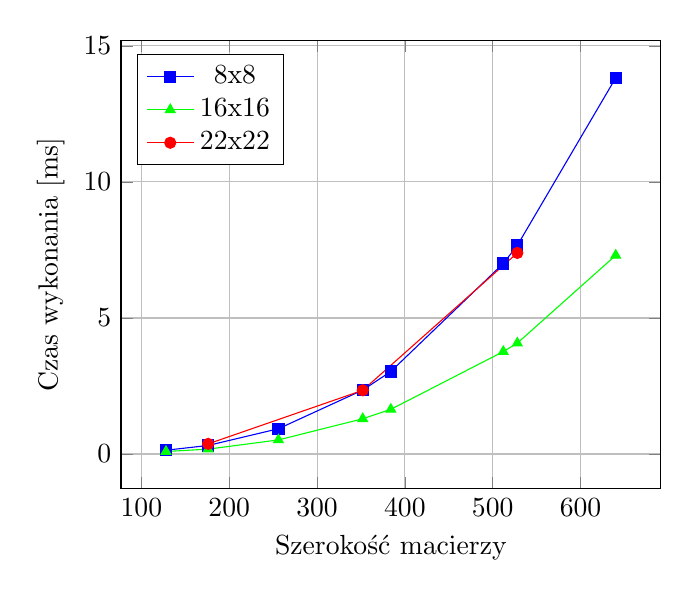
\begin{tikzpicture}
    \begin{axis}[
      xlabel=Szerokość macierzy,
      ylabel={Czas wykonania [ms]},
      legend pos=north west,
      grid=both
    ]

    \addplot[color=blue,mark=square*] coordinates {
      (128, 0.140)
      (176, 0.316)
      (256, 0.930)
      (352, 2.351)
      (384, 3.034)
      (512, 7.001)
      (528, 7.666)
      (640, 13.820)
    };
    \addlegendentry{8x8}

    \addplot[color=green,mark=triangle*] coordinates {
      (128, 0.093)
      (176, 0.181)
      (256, 0.519)
      (352, 1.297)
      (384, 1.642)
      (512, 3.764)
      (528, 4.075)
      (640, 7.301)
    };
    \addlegendentry{16x16}

    \addplot[color=red,mark=*] coordinates {
      (176, 0.374)
      (352, 2.343)
      (528, 7.389)
    };
    \addlegendentry{22x22}

    \end{axis}%
  \end{tikzpicture}%
\caption{Zależność pomiędzy czasem obliczeń a rozmiarem macierzy -- wersja 3.}
\end{figure}

\item \textbf{Ilość operacji zmiennoprzecinkowych na sekundę} \newline

\begin{table}[H]
\centering
\begin{tabular}{|c|c|c|c|}
\hline
\multirow{2}{*}{Rozmiar macierzy} & \multicolumn{3}{c|}{Rozmiar bloku} \\ \cline{2-4}
& 8x8 & 16x16 & 22x22 \\ \hline
128x128 & 29.857 & 45.291 & \textcolor{gray}{n/d}\\ \hline
176x176 & 34.491 & 60.169 & 29.138 \\ \hline
256x256 & 36.086 & 64.603 & \textcolor{gray}{n/d} \\ \hline
352x352 & 37.106 & 67.273 & 37.231 \\ \hline
384x384 & 37.322 & 68.970 & \textcolor{gray}{n/d} \\ \hline
512x512 & 38.341 & 71.314 & \textcolor{gray}{n/d} \\ \hline
528x528 & 38.402 & 72.246 & 39.844 \\ \hline
640x640 & 37.938 & 71.812 & \textcolor{gray}{n/d} \\ \hline
\end{tabular}
\caption{Ilosc operacji zmiennoprzecinkowych na sekundę (GFLOPS) -- wersja 3.}
\end{table}

\begin{figure}[H]
\centering
  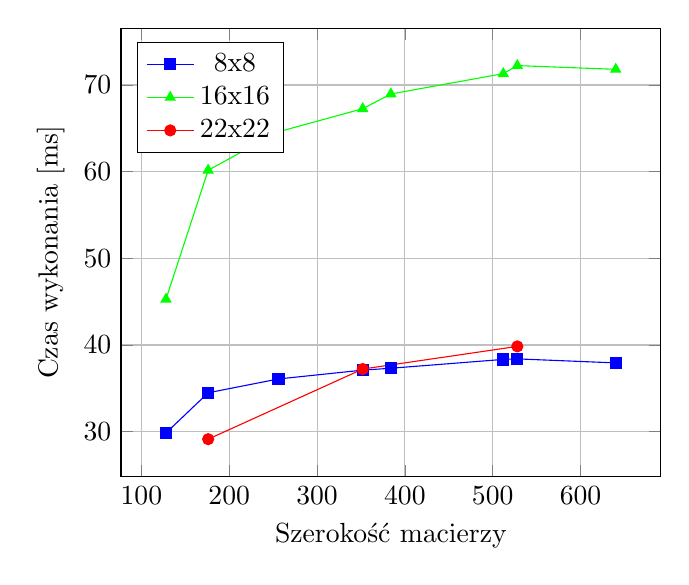
\begin{tikzpicture}
    \begin{axis}[
      xlabel=Szerokość macierzy,
      ylabel={Czas wykonania [ms]},
      legend pos=north west,
      grid=both
    ]

    \addplot[color=blue,mark=square*] coordinates {
      (128, 29.857)
      (176, 34.491)
      (256, 36.086)
      (352, 37.106)
      (384, 37.322)
      (512, 38.341)
      (528, 38.402)
      (640, 37.938)
    };
    \addlegendentry{8x8}

    \addplot[color=green,mark=triangle*] coordinates {
      (128, 45.291)
      (176, 60.169)
      (256, 64.603)
      (352, 67.273)
      (384, 68.970)
      (512, 71.314)
      (528, 72.246)
      (640, 71.812)
    };
    \addlegendentry{16x16}

    \addplot[color=red,mark=*] coordinates {
      (176, 29.138)
      (352, 37.231)
      (528, 39.844)
    };
    \addlegendentry{22x22}

    \end{axis}%
  \end{tikzpicture}%
\caption{Zależność pomiędzy ilością operacji zmiennoprzecinkowychna sekundę a rozmiarem macierzy -- wersja 3.}
\end{figure}

\item \textbf{Ilość instrukcji wykonanych na sekundę} \newline

\begin{table}[H]
\centering
\begin{tabular}{|c|c|c|c|}
\hline
\multirow{2}{*}{Rozmiar macierzy} & \multicolumn{3}{c|}{Rozmiar bloku} \\ \cline{2-4}
& 8x8 & 16x16 & 22x22 \\ \hline
128x128 & 0.1639 & 0.1562 & \textcolor{gray}{n/d}\\ \hline
176x176 & 0.16910 & 0.23896 & 0.12664 \\ \hline
256x256 & 0.1754 & 0.2622 & \textcolor{gray}{n/d} \\ \hline
352x352 & 0.17807 & 0.28408 & 0.15949 \\ \hline
384x384 & 0.1767 & 0.2926 & \textcolor{gray}{n/d} \\ \hline
512x512 & 0.1802 & 0.2948 & \textcolor{gray}{n/d} \\ \hline
528x528 & 0.18043 & 0.30390 & 0.17317 \\ \hline
640x640 & 0.1775 & 0.2989 & \textcolor{gray}{n/d} \\ \hline
\end{tabular}
\caption{Ilość instrukcji wykonana na sekundę (GIPS) -- wersja 3.}
\end{table}

\item \textbf{CGMA} \newline

\begin{table}[H]
\centering
\begin{tabular}{|c|c|c|c|}
\hline
\multirow{2}{*}{Rozmiar macierzy} & \multicolumn{3}{c|}{Rozmiar bloku} \\ \cline{2-4}
& 8x8 & 16x16 & 22x22 \\ \hline
128x128 & 120.471 & 546.133 & \textcolor{gray}{n/d} \\ \hline
176x176 & 129.067 & 516.267 & 354.253 \\ \hline
256x256 & 128.502 & 520.127 & \textcolor{gray}{n/d} \\ \hline
352x352 & 128.000 & 507.803 & 382.302 \\ \hline
384x384 & 128.000 & 515.580 & \textcolor{gray}{n/d} \\ \hline
512x512 & 127.626 & 514.008 & \textcolor{gray}{n/d} \\ \hline
528x528 & 127.765 & 510.593 & 380.668 \\ \hline
640x640 & 127.760 & 510.723 & \textcolor{gray}{n/d} \\ \hline
\end{tabular}
\caption{Stosunek ilości operacji zmiennoprzecinkowych do ilości operacji odczytu/zapisu z pamięci globalnej -- wersja 3.}
\end{table}

\end{enumerate}
